\documentclass{disser}
\hypersetup{
    pdfauthor={Карасюк Артём Денисович}, % Автор
    pdftitle={Выпускная квалификационная работа},    % Заголовок
    pdfsubject={Исследование алгоритмов генерации музыки с использованием искусственных нейронных сетей}
}

%%% Номер страницы сверху %%%
\usepackage{scrlayer-scrpage}

% для листинга программы
\usepackage{listings}

% для оформления картинок
\usepackage{graphicx}
\pagestyle{scrheadings}
\clearscrheadfoot
\cfoot[\pagemark]{\pagemark}

\onehalfspacing

\usepackage{caption}
\usepackage{pythonhighlight}
%\setcounter{tocdepth}{1}

%\addbibresource{mypapers.bib}
\begin{document}
%\ fontsize {5.0pt} {\ baselineskip} \ selectfont text
%\input{disser_tex/title}                  % Титульный лист

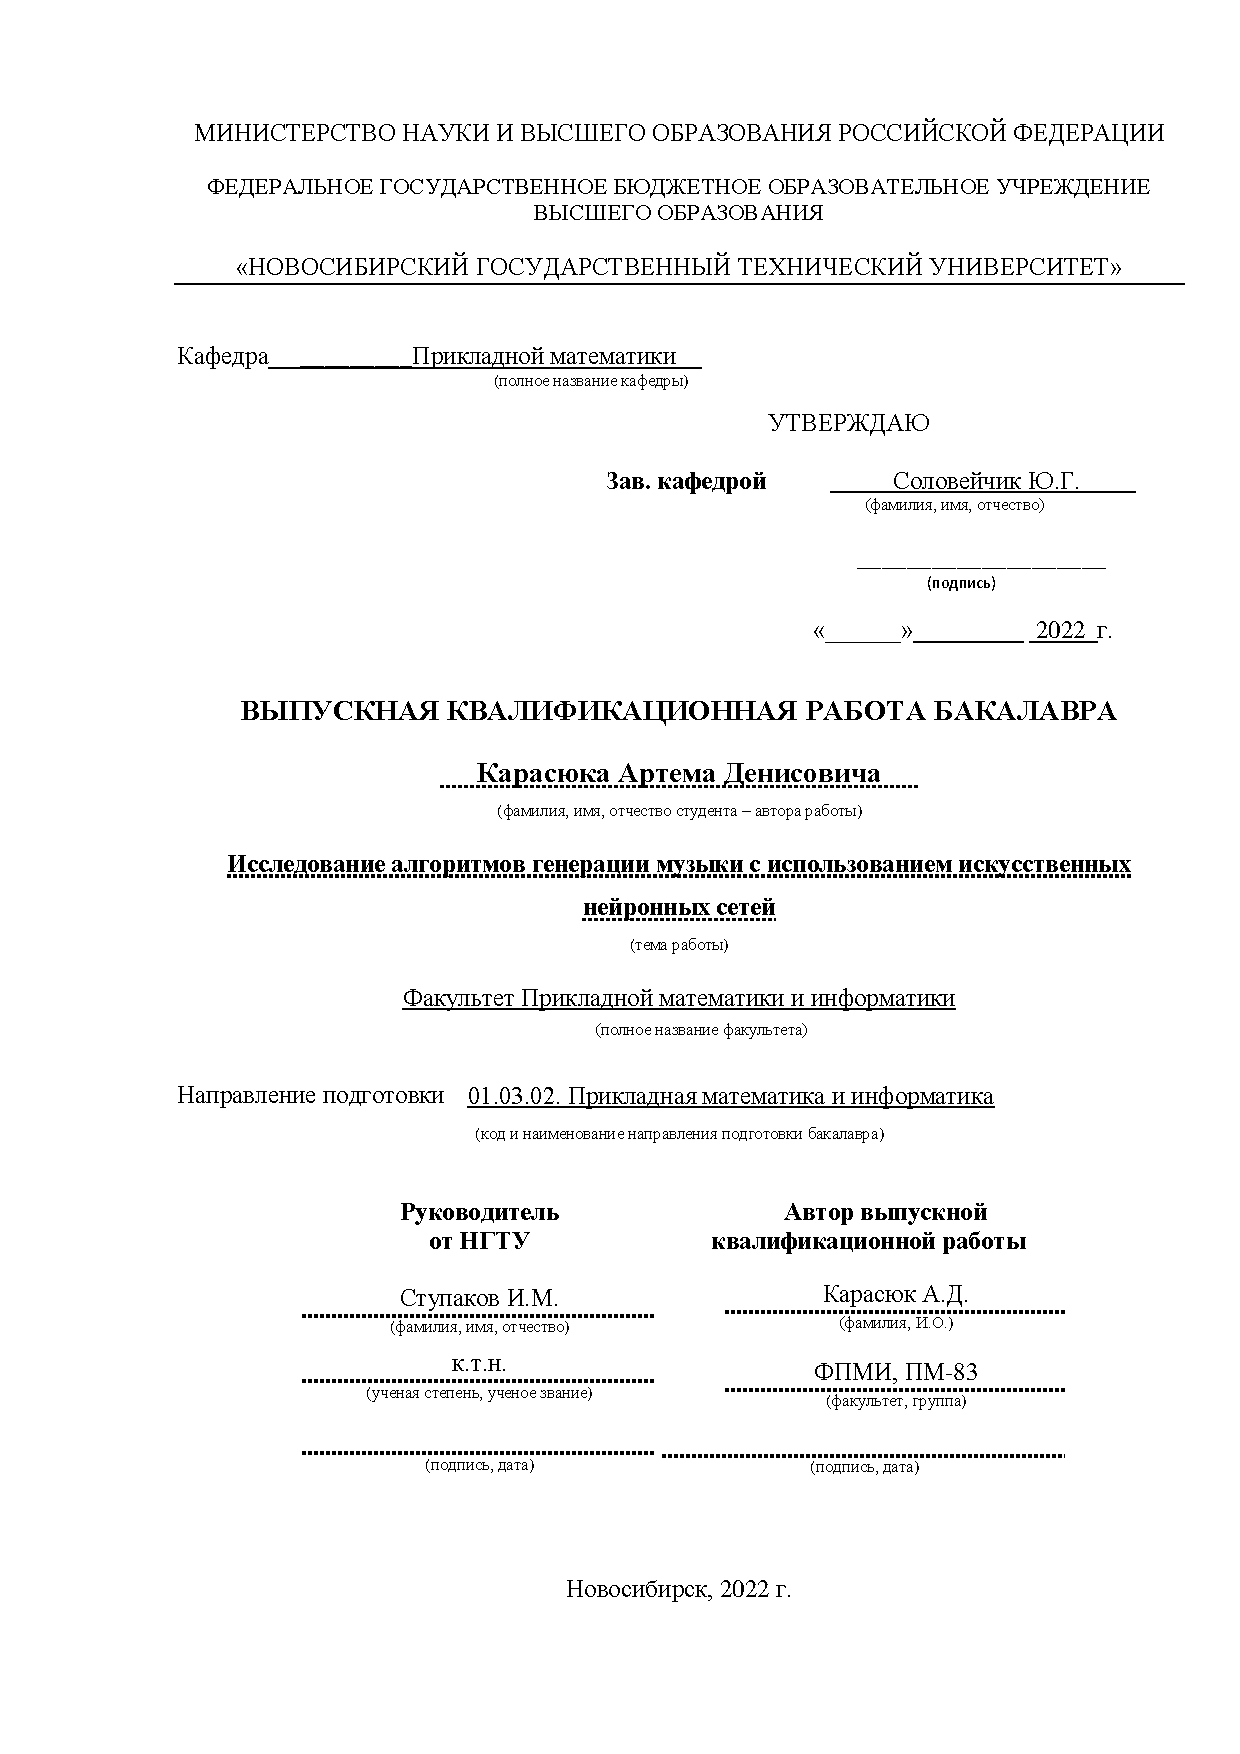
\includepdf{tex/titul/tituldiplom.pdf}
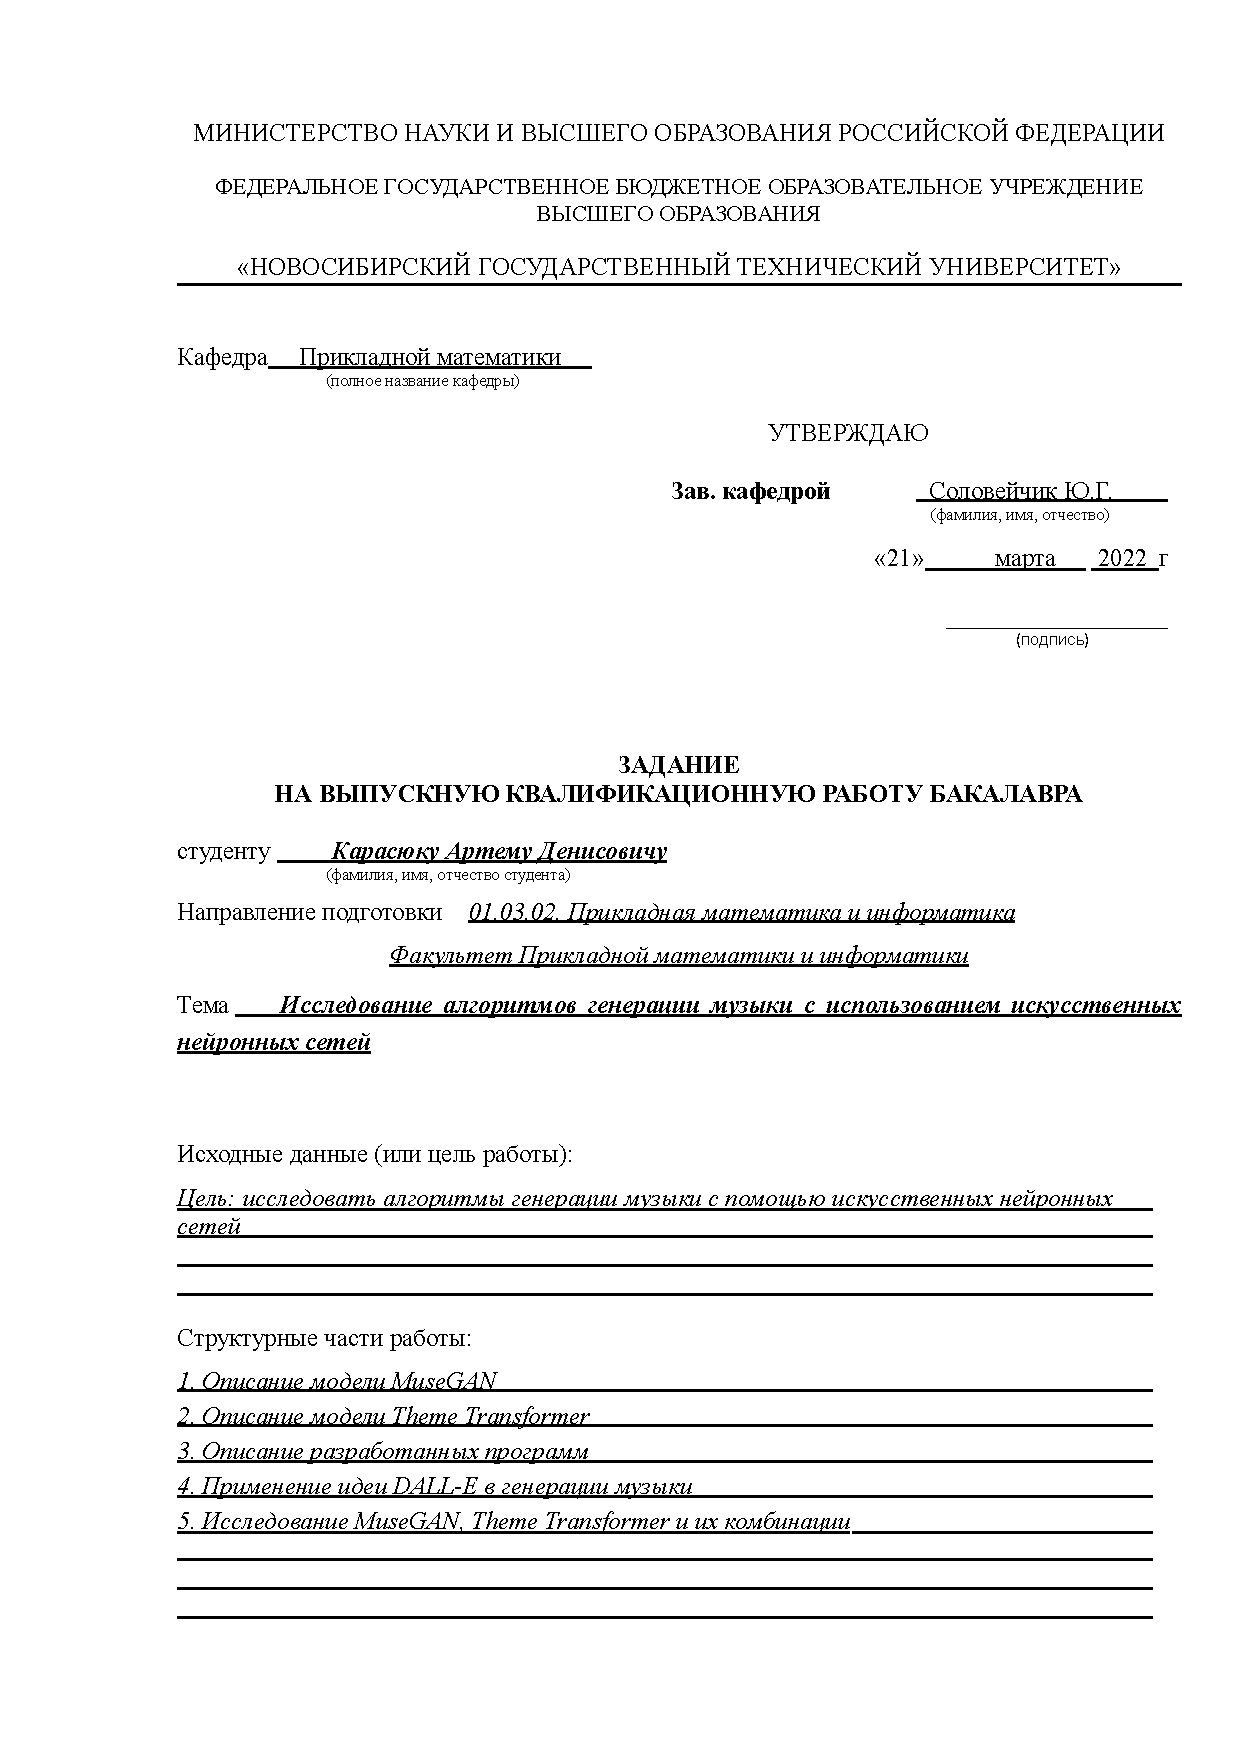
\includepdf[pages=-]{tex/titul/list_zadania.pdf}
\setcounter{page}{3}


\chapter*{АННОТАЦИЯ}
Отчет 54 с., 5 ч., 8 рис., 18 источников.

ГЛУБОКОЕ ОБУЧЕНИЕ, МУЗЫКА, MIDI-ФАЙЛЫ, НЕЙРОННЫЕ СЕТИ, АРХИТЕКТУРА ТРАНСФОРМЕРОВ, ГЕНЕРАТИВНО-СОСТЯЗАТЕЛЬНЫЕ НЕЙРОННЫЕ СЕТИ, ГЕНЕРАЦИЯ МУЗЫКИ

Объектом исследования являются алгоритмы генерации музыки, использующие нейронные сети.

Цель работы – проведение сравнительного анализа алгоритмов генерации музыки с использованием нейронных сетей для выявления процесса обучения и разнообразности результата.

В процессе работы проводилось изучение архитектур нейронных сетей MuseGAN и Theme Transformer, которые успешно генерировали композиции. Так же была рассмотрена такая проблема, как разнообразие генерируемых композиций с помощью классификаторов жанров. 

В результате исследования алгоритмов для генерации музыки были исследованы такие модели, как MuseGAN и Theme Transformer. В результате исследований было выявлено, что данные модели генерируют с точки зрения классификаторов жанров одно и то же (первый и второй классификаторы используют MP3 и MIDI файлы для анализа соответственно).

Также был предложен новый вариант алгоритма, который подразумевает под собой комбинацию данных моделей — MuseGAN генерирует начало композиции, а Theme Transformer её продолжает. Такое решение генерирует более разнообразные композиции (с точки зрения первого классификатора). Был создан сайт для прослушивания результатов генерации и разработан программный модуль на языке Python для исследований. 

\thispagestyle{empty}

\tableofcontents                          % Оглавление
\addtocontents{toc}{\protect\thispagestyle{empty}}
\thispagestyle{empty}

\addchap{ВВЕДЕНИЕ}
	Нейронные сети на данный момент применяются во многих областях. Их применяют для распознавания образов, синтеза речи и её распознавания и т.д. Данная область растёт очень быстро и решает большой круг задач, которые раньше могли решить только люди. 

Так же нейронные сети могут применяться и в задаче создания музыки. Для этого необходимо знать некоторые правила создания композиций. Здесь можно привести пример с говорением. В устной речи тоже необходимо знать правила языка для того, чтобы грамотно излагать мысли. И в той, и в другой ситуации при нарушении правил могут возникнуть проблемы с восприятием. Если человек скажет что-то неграмотно, то другой может его не понять. Если будет сыграна нота, не относящаяся к тональности, то это будет 'резать' слух. 

Музыка -- это искусство, обладающее периодичностью, а потому требующее временной модели. Музыка имеет иерархическую структуру -- высокоуровневые строительные блоки (фразы) состоят из более мелких рекуррентных шаблонов (тактов). Когда люди слушают музыку, то они уделяют внимание структурным шаблонам, связанным с согласованностью, ритмом, напряжением и потоками эмоций. Таким образом, механизм учета временной структуры имеет решающее значение.

Музыка обычно состоит из нескольких инструментов/дорожек. Современный оркестр, как правило, включает в себя четыре различные инструментальные секции: духовые, струнные, деревянные духовые и перкуссия; рок группа часто состоит из баса, ударных, гитары и вокала. Эти дорожки тесно связаны и разворачиваются во времени независимо.

Ноты часто образуют аккорды, арпеджио или мелодии в полифонической музыке. В связи с этим введение хронологического порядка нот не совсем естественно, т. к. в композиции партия одного инструмента может дополнять партию другого. Таким образом, успехи в создании текстов на естественном языке и монофонической музыки не могут в полной мере распространяться на генерацию полифонической музыки.

Генерация музыкального контента может быть необходима для: музыкальных стриминговых сервисов под настроение и пожелания пользователя, музыкального сопровождения подкастов, видеороликов, игр и пр., создания идеи композиции, продолжения существующей композиции и т.д.

Генерация музыки уже успешно применяется в сервисах для предоставления композиций под пожелания пользователя \cite{brainfm}.

В данной работе рассмотрены алгоритмы генерации музыки с помощью генеративно-состязательных нейронных сетей и трансформеров. Так же были изучены данные модели на разных этапах тренировки (глава \ref{chapter4}) и было проверено эвристическое правило отбора 'лучших' композиций с помощью классификаторов жанров (глава \ref{chapter3}). 

В рамках анализа архитектуры (главы \ref{chapter1} и \ref{chapter2}) исследована каждая из моделей (MuseGAN, Theme Transformer соответственно) и выявлены их недостатки.
           % Введение

\chapter{~ОПИСАНИЕ МОДЕЛИ MUSEGAN}\label{chapter1}
%	\input{disser_tex/stateofart} % Вставить куда-нить!
	В данной главе рассмотрена архитектура генеративно-состязательной нейронной сети MuseGAN. Данная модель может использоваться для генерации с нуля и для продолжения композиции.

\section{ПРЕДСТАВЛЕНИЕ ДАННЫХ}

    В статье предлагается использовать представление в виде фортепианного ролла (рисунок \ref{fig:midi}) с несколькими дорожками \cite{musegan}. На данном рисунке горизонтальная прямая представляет собой время, а вертикальная -- высоту ноту (от меньшей к большей). Чёрный пиксель значит, что определённая нота сыграна в данный временной промежуток. Данная нейронная сеть моделирует полифоническую музыку с несколькими дорожками.
    
    \begin{figure}
        \centering
        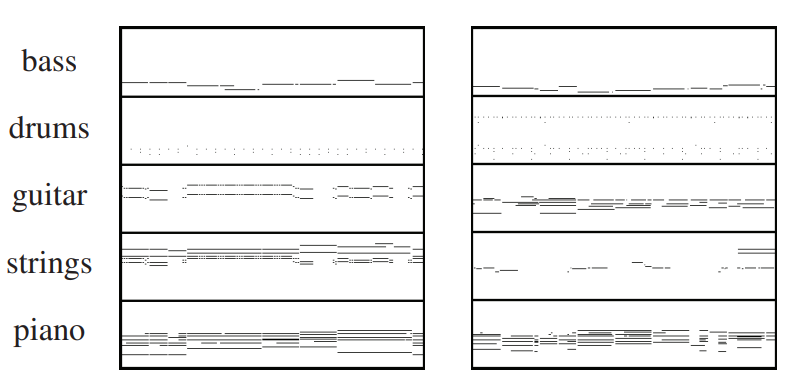
\includegraphics[scale=0.7]{tex/png/midi-example.png}
        \caption{Пример композиции с 5-ю дорожками \cite{musegan}}
        \label{fig:midi}
    \end{figure}
    
    
    Представление в виде фортепианного ролла — это бинарная матрица, отражающая наличие нот на различных временных шагах. 
    Горизонтальная ось — время, вертикальная ось — высота ноты (от низких к высоким). 
    При иллюстрации данной матрицы черный пиксель показывает, что определенная нота звучит на конкретном временном шаге. 
    Говоря формальным языком, фортепианный ролл с $\mathbf{M}$ дорожками одного такта представляется как тензор $ \mathbf{x} \in {0,1}^{R \times S \times M}$, где $ \mathbf{R} $ и $ \mathbf{S} $ обозначают число временных шагов в такте и число кандидатов в ноты соответственно. 
    Фортепианный ролл с $ \mathbf{M} $ дорожками из $ \mathbf{T} $ тактов представляется как $ \vec{x} = \{\vec{x}^{(t)}\}^T _ {t=1} $, где $ \vec{x}^{(t)} \in {0,1}^{R \times S \times M} $ обозначение фортепианного ролла с несколькими дорожками такта $ t $.
    
    Стоит заметить, что фортепианный ролл каждых такта и дорожки, как и для настоящих, так и для сгенерированных данных, представлен в виде матрицы фиксированного размера, что позволяет использовать сверточные нейронные сети.

\section{МОДЕЛИРОВАНИЕ НЕЗАВИСИМОСТИ ДОРОЖЕК}

    Существуют два стандартных способа создания музыки; рассмотрим их далее.
    \begin{enumerate}  
    \item Группа музыкантов, играющая на различных инструментах, может создавать музыку с помощью импровизации без подготовки и соглашений. Данный процесс известен как джем-сешн.
    \item Предоставление услуг композитора, который может выстроить композицию, обладая знаниями о гармонической структуре и доступном инструментарии. Далее музыканты могут сыграть уже сочиненную музыку.
    \end{enumerate}
    
    В архитектуре MuseGAN используется одновременно 3 модели, соответствующих этим композиционным подходам.
    
    Джем-модель (рисунок \ref{fig:jam}) устроена следующим образом: несколько генераторов работают независимо и создают музыку для собственных дорожек из приватного случайного вектора $\vec{z}_i $, $i=1,2,...,M$, где $M$ -- число дорожек. Эти генераторы получают обратную связь (через обратное распространение ошибки) от различных дискриминаторов.
    
    \begin{figure}
        \centering
        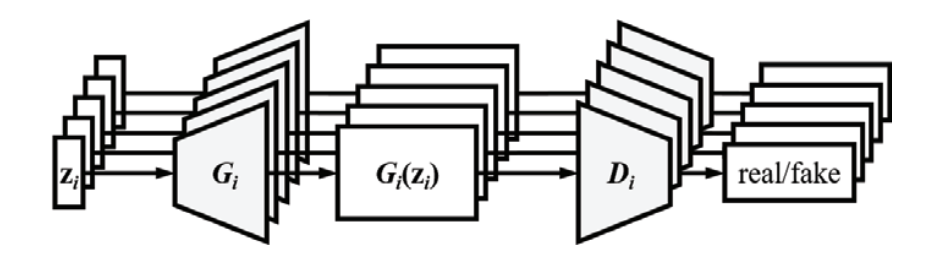
\includegraphics[scale=0.4]{tex/png/jamm.png}
        \caption{Представление джем-модели \cite{musegan}}
        \label{fig:jam}
    \end{figure}
    
    Модель-композитор (рисунок \ref{fig:composer}) включает в себя один генератор, который создает многоканальный фортепианный ролл, где каждый канал представляет определенную дорожку. 
    Данная модель требует только один общий случайный вектор $z$ (который может быть интерпретирован как замысел композитора) и один дискриминатор, который проверяет все $M$ вместе для того, чтобы определить, является ли вход настоящим или поддельным.
    
    \begin{figure}[h]
        \centering
        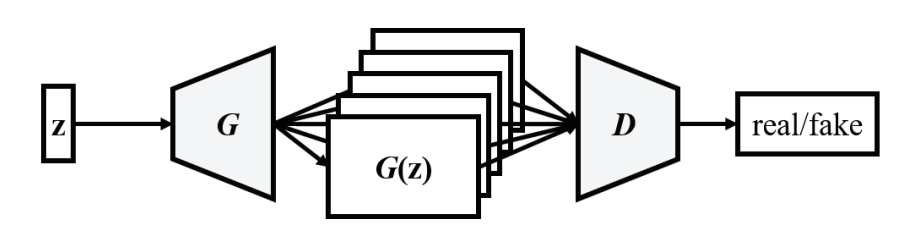
\includegraphics[scale=0.4]{tex/png/composer.png}
        \caption{Представление модели композитора \cite{musegan}}
        \label{fig:composer}
    \end{figure}
    
    При объединении идей джем-модели и модели композитора получается гибридная модель (рисунок \ref{fig:hybrid}). Каждый из $M$ генераторов принимает на вход “внутренний” случайный вектор $z$ и “внешний” случайный вектор. Роль “внутреннего” случайного вектора заключается в координации генераторов, как это делает композитор с музыкантами. Более того, только один дискриминатор оценивает все $M$ дорожек.
    
    \begin{figure}
        \centering
        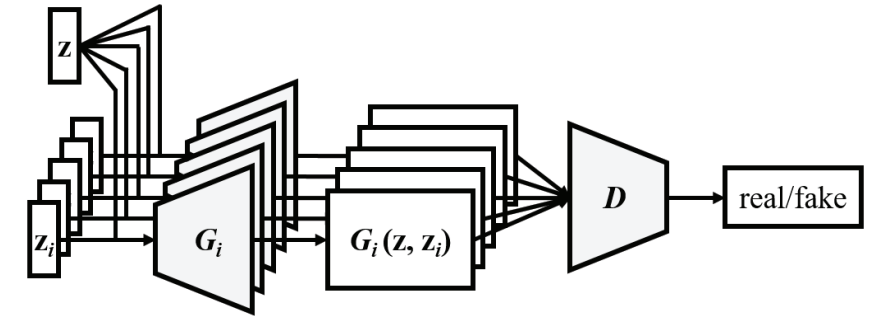
\includegraphics[scale=0.4]{tex/png/hybrid.png}
        \caption{Представление гибридной модели \cite{musegan}}
        \label{fig:hybrid}
    \end{figure}
    
    Главное отличие между моделью-композитором и гибридной — это гибкость. В гибридной модели можно использовать различные архитектуры нейронных сетей (т.е. варьировать число слоев, размер фильтра) и неодинаковые входы для каждого из генераторов. Таким образом, можно, например, менять процесс генерации одной определенной дорожки без потери связи между ними.

\section{МОДЕЛИРОВАНИЕ ВРЕМЕННОЙ СТРУКТУРЫ}
    Результатом генерирования описанных выше моделей является композиция с несколькими дорожками без согласованности между тактами. Для решения данной проблемы необходима временная модель для генерации музыки длиной в несколько тактов.
    
    Первый метод нацелен на генерацию музыкальных фраз фиксированной длины, что 
    достигается путем просмотра последовательности тактов. Генератор (рисунок \ref{fig:model_architecture}) состоит из двух частей: генератора временной структуры $G_{temp}$ и генератора тактов $G_{bar}$.
    
    \begin{figure}[h]
        \centering
        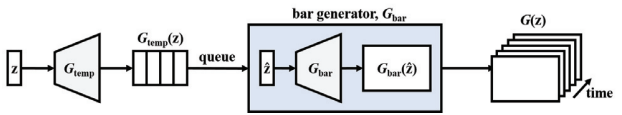
\includegraphics[scale=0.7]{tex/png/architecture_from_stratch.png}
        \caption{Архитектура модели для учёта временной структуры \cite{musegan}}
        \label{fig:model_architecture}
    \end{figure}
    
    $G_{temp}$ отображает вектор шума $z$ в некоторую последовательность латентных векторов $\vec{z} = \{ \vec{z}^{(t)} \} ^ T _ {t=1}$. Результирующий вектор (он несёт в себе временную информацию) затем использует $G_{bar}$ для последовательной генерации фортепианных роллов (такт за тактом):
    $$ G(z) = \{ G_{bar} \} ^ T _ {t=1}. $$
    
    Второй метод предполагает, что последовательность тактов $\vec{y}$ одной определённой дорожки задаётся человеком, и пытается выучить лежащую в основе временную структуру и генерировать оставшиеся дорожки. Зависимый от других дорожек генератор $G^{o}$ создает такты один за другим с помощью условного генератора тактов $G^o_{bar}$. Фортепианные роллы оставшихся дорожек такта $t$ генерируются $G^o_{bar}$, который принимает на вход условие $\vec{y}$ и зависящий от времени случайный шум ${\vec{z}} ^ {(t)}$.
    
    Для достижения такой условной генерации при работе с ситуациями большой размерности обучается энкодер $E$ для отображения $\vec{y}^{(t)}$ в пространство $\vec{z}^{(t)}$. Итоговая процедура выглядит следующим образом:
    $$ G^o(\vec{z}, \vec{y}) = \{G^o_{bar}(\vec{z}^{(t)}, E(\vec{y}^{(t)}))\}^T_{(t=1)}. $$
    
    Кодировщик будет извлекать “внутренние” признаки вместо “внешних”, т.к. “внешняя” дорожка не особо полезна для генерации остальных дорожек.

\section{АРХИТЕКТУРА МОДЕЛИ}
    
    MuseGAN представляет собой объединение и расширение представленных выше моделей (рисунок \ref{fig:full_musegan}). Рассмотрим более подробно данную архитектуру. 
    
    \begin{figure}[h]
        \centering
        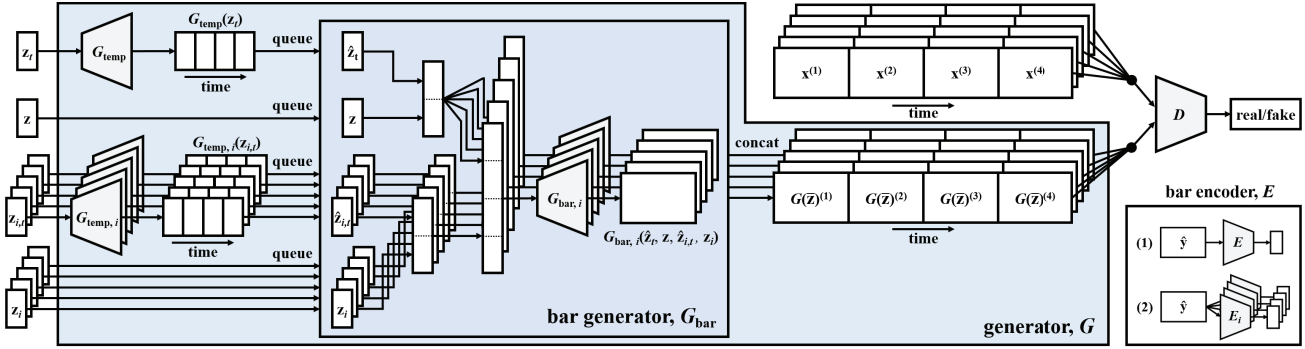
\includegraphics[scale=0.38]{tex/png/full_musegan.png}
        \caption{Полная архитектура модели генератора MuseGAN \cite{musegan}}
        \label{fig:full_musegan}
    \end{figure}
    
    Вход ($\vec{z}$) состоит из четырёх частей: 'внутренние'  независящие от времени случайные векторы $z$, 'внешние'  зависящие от времени векторы $z_i$, 'внутренние'  зависящие от времени случайные векторы $z_t$ и 'внешние'  зависящие от времени случайные векторы ${z_{i,t}}$. Для $i$-й дорожки ($i$ = 1,2, … , $M$), общий генератор временной структуры $G_{temp}$ и приватный генератор временной структуры $G_{temp, i}$ принимают на вход зависящие от времени случайные вектора $z_{t}$ и $z_{i,t}$ соответственно, и каждый из генераторов производит ряд из латентных векторов, содержащих “внутреннюю” и “внешнюю” временную информацию. Полученные ряды конкатенируют и поступают на вход генератору тактов, который последовательно создает фортепианные роллы. Процедуру генерации можно описать следующей формулой:
    $$G(\vec{z}) = \{G_{bar,i} (z, G_{temp}(z_{t})^{(t)}, z_{i}, G_{temp,i}(z_{i,t})^{(t)}) \} ^ {M,T} _ {i,t=1},$$
    где $G$ и $D$ реализованы как глубокие сверточные сети. $G$ прежде всего наращивает длительность ноты, а затем увеличивает высоту ноты, в то время как $D$ делает наоборот.
    
\section{ОЦЕНКА РАБОТЫ МОДЕЛИ}
    Для оценки работы модели можно использовать следующие метрики:
    \begin{enumerate}
        \item Количество пустых тактов к количеству всех тактов (в процентах).
        \item Количество используемых нот на такт (от 0 до 12).
        \item Количество правильных нот (в процентах). Правильной нотой считается та нота, которая не короче трёх временных шагов (то есть 32-ая нота). Данная метрика показывает как сильно композиция в результате фрагментирована.
        \item Ритмический паттерн: коэффициент нот, которые удовлетворяют 8-ми или 16-ти нотным паттернам, как обычно бывает в рок-композициях с размером 4/4.
        \item Тональное расстояние \cite{tonal-distance}. Оно измеряет гармоничность между парой тактов. Чем больше эта метрика, тем меньше композиция согласуется с собой.
    \end{enumerate}
    
    Для того, чтобы оценить итоговую модель -- считается статистика по данным значениям на реальных данных и потом они сравниваются с теми, которые посчитаны на данных, которые выдаёт генератор. В течении тренировки генератор должен создавать композиции, всё больше сближаясь к тренировочным данным.
    
    Недостатки модели были выявлены и описаны в главе исследований.
	
\chapter{~ОПИСАНИЕ МОДЕЛИ THEME TRANSFORMER}\label{chapter2}
	В данной главе рассмотрена искусственная нейронная сеть, которая использует архитектуру трансформера для генерации продолжения композиций.
Перед тем как приступить к изложению архитектуры Theme Transformer \cite{theme}, стоит объяснить архитектуру классических трансформеров, и только потом перейти к его модификации.

\section{ОПИСАНИЕ АРХИТЕКТУРЫ ТРАНСФОРМЕРОВ}
\subsection{ОСНОВНАЯ ИДЕЯ МОДЕЛИ}
    Большинство seq2seq моделей основаны на больших рекуррентных или сверточных нейронных сетях, которые включают в себя кодировщик и декодер. Лучшего результата таких моделей можно достичь, если кодировщик и декодер будут соединены между собой механизмом внимания. В статье представлена модель трансформера, основанного на архитектуре модели seq2seq, имеющий механизм внимания, что имеет преимущества \cite{attention}. Во-первых, нет необходимости иметь свёрточные и рекуррентные слои. Во-вторых, обучение модели может проходить параллельно. В-третьих, модели требуется меньше времени на тренировку.
    
    Данная архитектура (рисунок \ref{fig:transformer}) является модификацией архитектуры seq2seq модели. Модификация заключается в наличии в каждом кодировщике механизма самовнимания (self-attention) и классического механизма внимания (attention) между кодировщиком и декодером.
    
    \begin{figure}
        \centering
        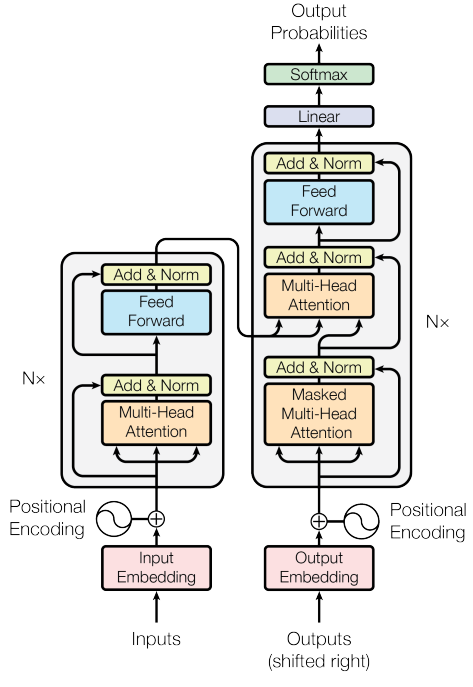
\includegraphics[scale=1.2]{tex/png/transformer.png}
        \caption{Архитектура трансформера \cite{attention}}
        \label{fig:transformer}
    \end{figure}
    
    Недостатком seq2seq модели является скрытый вектор состояния фиксированного размера, что не позволяет сжать много информации из ввода, особенно если он длинный.

    Механизм внимания позволяет отказаться от основной идеи рекуррентных и сверточных нейронных сетей, тем самым ускорив обучение нейронной сети, т. к. появляется возможность тренировать их независимо.

\subsection{АРХИТЕКТУРА}
    Кодировщики и декодеры представляют собой некоторый стек идентичных слоёв. 
    
    Каждый слой в кодировщике состоит из двух подслоёв. Первым слоем является multi-head self-attention механизм, а второй -- полносвязный. После них расположен слой нормализации, который принимает вход с предыдущего слоя (остаточная связь), то есть $ LayerNorm(x + Sublayer(x)) $, где $ Sublayer(x) $ -- это функция, которая реализуется слоем (в нашем случае это или multi-head self-attention, или полносвязный слои). Чтобы было легче пользоваться остаточной связью, каждый слой формирует вектор одинаковой размерности. 
    
    Если у кодировщика слой состоит из 2 подслоёв, то к декодеру добавляется третий multi-head attention, который принимает выход из кодировщика. Также этот слой принимает на вход результат слоя самовнимания, который маскирует некоторые позиции и, как следствие, игнорируются моделью. Эта маскировка и смещение выходного вектора на одну позицию гарантирует, что прогноз на $i$-й позиции зависит только от позиций меньших $i$.

\subsection{МЕХАНИЗМ ВНИМАНИЯ}
    Механизм внимания оперирует 3-я элементами: $Q$ -- запрос размерности $ d_k $, $K$ -- ключ размерности $ d_k $ и $V$ -- значение размерности $ d_v $.
    
    Данные элементы получаются в результате перемножения исходного вектора на матрицы $W^Q, W^K, W^V$ соответственно. Они формируются во время обучения нейронной сети и являются некоторым скрытым состоянием.
    
    Данный механизм в качестве элементов $Q, K, V$ может иметь вектора или матрицы.
    
    Вектор или матрица (в зависимости от вида механизма) внимания вычисляется следующим образом:
    $$ Attention(Q, K, V) = softmax(\frac{QK^T}{\sqrt{d_k}})V, $$
    где softmax -- функция вида $f(x) = \frac{\exp{x_k}}{\sum \exp{x_i}}$, $\frac{1}{\sqrt{d_k}}$ -- нормирующий коэффициент, который позволяет увеличить градиент (отчасти решая проблему исчезающих градиентов).
    
\subsection{MULTI-HEAD ATTENTION}
    Входной вектор разбивается на h частей. Таким образом, у каждого механизма внимания размерность следующая: $d_k = d_v = d_{model} / h$.
    
    В декодере один из таких механизмов должен принимать выход от кодировщика, ожидая от него $K$ и $V$. 
    
    Благодаря разбиению одного большого механизма внимания на несколько маленьких (в оригинальной статье разбивается на 8 частей) позволяет модели фокусироваться на разных частях входа \cite{attention}. Таким образом, модель способна выявлять связи между различными позициями.
    Также благодаря этому увеличивается количество подпространств. Это позволяет каждому маленькому механизму концентрироваться только на связи отдельных позиций.
    
    После того, как вектор прошёл через данный механизм, нам необходимо вернуться к исходному пространству векторов, так как полносвязный слой ожидает на вход вектор размерности $d_{model}$. Чтобы этого добиться, нам необходимо конкатенировать вектора с каждой головы (маленькая часть) и умножить на общую матрицу $W^O$ (формируется во время обучения).
    
    Формализуя описанные шаги, получаем:
    $$ MultiHead(Q, K, V) = Concat(head_1, ..., head_h)W^O, $$
    где $head_i = Attention(QW_{i}^Q, KW_{i}^K, VW_{i}^V)$, $Concat$ -- функция конкатенации векторов в один, $W_i^Q \in R^{d_{model} \times d_k}$, $W_i^K \in R^{d_{model} \times d_k}$, $W_i^V \in R^{d_{model} \times d_v}$, $W^O \in R^{hd_v \times d_{model}}$.
    
\subsection{СЕТИ ПРЯМОГО РАСПРОСТРАНЕНИЯ, ЗАВИСЯЩИЕ ОТ ПОЗИЦИИ}
    Каждый блок декодера и кодировщика содержит в себе полносвязную сеть прямого распространения, которая идентично применяется ко всем позициям отдельно. В нём содержится две линейные трансформации с функцией активации ReLU:
    $$ FFN(x) = max(0, xW_1 + b_1)W_2 + b2. $$
    
    Линейные преобразования одинаковы для разных позиций, но они имеют разные параметры от слоя к слою, что эквивалентно использованию двух сверточных слоёв с размером ядра 1. 
    

\section{ОПИСАНИЕ РАБОТЫ THEME TRANSFORMER}
    В последние годы стала популярна архитектура трансформеров, т.к. в ней используется механизм внимания (в частности self-attention), который обеспечивает модели гораздо большую память по сравнению с рекуррентной нейронной сетью.
    
    Такие модели всё чаще используют для генерации музыки. Популярным подходом, обуславливающим процесс генерации, является принятие входных данных как последовательности инициализации для дальнейшей работы декодера. 
    Данный метод не гарантирует развития и повторения элементов исходных данных в генерированном продолжении. 
    Однако данная модель, описанная далее, использует альтернативный подход ко входным данным. При добавлении входной последовательности система трактует её как тематический материал, который должен многократно проявляться в результате генерации.
    
    Приведённый выше подход реализуется с помощью метода, основанный на глубоком обучении. Он использует изучение контрастного представления и кластеризацию для автоматического извлечения тематических материалов из музыкальных произведений в обучающих данных. Также он необходим для выявления в композиции основной темы. Также модифицирована архитектура декодера: self-attention идёт параллельно cross-attention, после чего применяется операция XOR, полученные вектора суммируются и нормализуются. Данная модификация используется для более эффективного учёта заданного тематического материала в процессе генерации.

    По итогу данная модель может использоваться для генерации произведений с нуля или с подсказкой, предоставленной пользователем, для создания продолжения. 
    
    Генерация произведений с нуля возможна благодаря тому, что обучается модель трансформера, которая состоит из двух частей. Кодировщик обеспечивает некоторое внутреннее представление композиции, а декодер может взять выход с кодировщика или случайное начальное значение и генерировать продолжение.
    
    Такая архитектура позволяет изучать языковую модель музыки без правил, созданных вручную, и генерировать уникальные и разнообразные произведения, которые внутренне согласованы. Однако эта стратегия не гарантирует, что модель будет повторять или развивать данное условие или ранее созданный материал. Более того, поскольку музыкальное произведение постоянно расширяется, влияние начального фрагмента со временем уменьшается, т.е. модель теряет направление.
    
    \subsection{ПОДХОД К ОБУЧЕНИЮ}
    Рассмотрим подход к данным. Существуют уже готовые наборы данных и необходимо обучить модель, которая используя основную тему генерирует продолжение. И так как выделять самостоятельно в огромном наборе данных основную тему было бы крайне затратно -- реализован алгоритм, который делает это сам. 
    
    Суть алгоритма заключается в том, чтобы разбить исходную композицию на сегменты и получить их представление через кодировщик. Т. к. потом идёт работа с векторами -- в таком случае можем использовать алгоритм кластеризации (в оригинальной статье используется DBSCAN) для обнаружения наибольшего кластера. Первое вхождение в данный кластер и будет являться основной темой, а размер кластера будет указывать на частоту его появления в генерируемой композиции.
    
    После такой разметки данных модель обучается с использованием основной темы генерировать исходную композицию.
    
    \subsection{АРХИТЕКТУРА THEME TRANSFORMER}
    Архитектура Theme Transformer (рисунок \ref{fig:theme_transformer}) является модификацией исходного трансформера.
    В декодере изменён модуль внимания, в котором теперь cross attention не использует выход из самовнимания, а идёт параллельно. 
    При этом в архитектуре используется операция XOR для двух векторов. 
    После этого они подаются на вход нормировки и в сеть прямого распространения.
    
    Данное изменение улучшает работу при генерировании с условием \cite{theme}. 
    \begin{figure}[h]
        \centering
        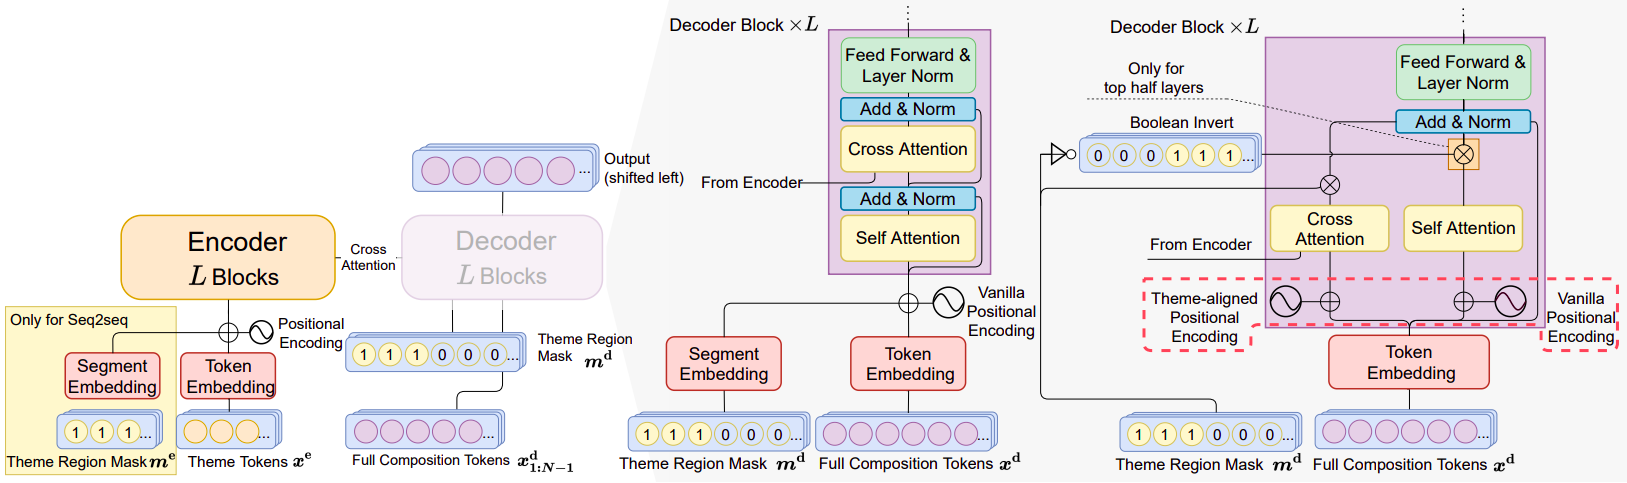
\includegraphics[scale=0.3]{tex/png/theme_transformer.png}
        \caption{Архитектура Theme Transformer с наглядной демонстрацией отличий от классической seq2seq модели \cite{theme}}
        \label{fig:theme_transformer}
    \end{figure}
    
    \subsection{ПРОЦЕСС ОБУЧЕНИЯ}
    
    Обучение происходит на основе набора данных POP909, состоящего из популярных композиций, которые исполняют только на пианино. Они созданы профессиональными музыкантами. Каждый MIDI-файл состоит из трёх дорожек: MELODY (основная мелодия, которую исполняет вокал), BRIDGE (второстепенная мелодия или основной инструмент) и PIANO (основной аккомпанемент). Для изучаемой модели дорожка BRIDGE была опущена, т. к. включает в себя функции и MELODY, и PIANO. Игнорирование названной дорожки не сильно ухудшает качество исходных треков \cite{theme}.
    
    Были выбраны композиции с тактовым размером 4/4. Также ноты были выравнены таким образом, чтобы время их начала и длительность были кратны 1/4 доли. Таким образом были проигнорированы сложные приёмы построения ритмических рисунков с целью упрощения работы модели. Также были убраны композиции с модуляцией.
    
    В итоге набор состоит из 713 композиций. 4\% оставлены для тестирования (29 файлов), а остальные -- для обучения модели. 

    Рассматриваются три вида токенов для представления каждой песни из POP909: для описания ноты, для описания звучания по времени, для описания начала и конца `основной темы`.
    
    Каждая нота в песне состоит из трёх лексем: высота (NOTE-PITCH; от D0 до G9), длительность (NOTE-DURATION; от 1/4 до 16 долей, кратная 1/4) и сила исполнения (NOTE-VELOCITY; от 1 до 126). Также необходимо принимать несколько дорожек; соответственно, будет использован отдельный токен, обозначающий мелодию или аккомпанемент. Например, чтобы описать высоту ноты дорожки MELODY в C5, используется токен NOTE-PITCH:MELODY:C5. 
    
    Для представления звучания по времени используются токены, связанные с метрикой. BAR отмечает начало нового такта, равномерно разделенного на 16 частей. SUBBEAT указывает время начала ноты среди этих 16 возможных позиций в такте. TEMPO описывает скорость песни на уровне битов и принимает значения от 17 до 194 ударов в минуту с интервалом 3. 
    
    Всего словарь для фортепиано содержит 730 уникальных токенов. Среди них нет токена конца композиции, т.к. используется последовательность из 512-ти токенов на вход вместо передачи всей композиции, что позволяет генерировать продолжение бесконечно.
    
    В тренировочном наборе данных композиции имеют в среднем 95 тактов, что составляет 5 249 токенов на песню с использованием представления фортепиано. Соответственно, последовательность из 512 токенов, используемая при обучении модели, содержит в среднем около девяти тактов. Фрагмент с основной темой из двух тактов содержит в среднем 122 токена.
    


\chapter{~ОПИСАНИЕ РАЗРАБОТАННЫХ ПРОГРАММ}\label{chapter31}
    В данной главе представлена разработанная программа, с помощью которых проводилось исследование разработанных моделей.

Помимо программы был создан сайт для прослушивания сгенерированных результатов моделями и просмотра агрегированных результатов классификации по жанрам. Данный сайт находится по адресу https://polisika.github.io/generate\_music\_analysis/.

В приложении А представлен текст программы для исследований, с помощью которой были получены результаты, представленные в главе исследований. Так же он представлен в удалённом репозитории по адресу https://github.com/Polisika/generate\_music\_analysis.

Так же был создан репозиторий с исходным кодом модифицированного модуля Theme Transformer. Данный репозиторий является копией исходного с некоторыми модификациями, необходимыми для распределённого обучения на нескольких видеокартах. Просмотреть его можно по адресу https://github.com/Polisika/ThemeTransformer/tree/torch-lightning.

\section{ОБЩИЕ СВЕДЕНИЯ}
Программный комплекс для исследования моделей MuseGAN и Theme Transformer.

Программное обеспечение, необходимое для функционирования: 
\begin{itemize}
    \item интерпретатор python 3.10;
    \item сторонние пакеты librosa, sklearn, pandas, catboost, seaborn, mido, torch, pypianoroll, numpy.
\end{itemize}

\section{ФУНКЦИОНАЛЬНОЕ НАЗНАЧЕНИЕ}

\emph{define\_model.py} -- скрипт, содержащий код для определения генератора модели MuseGAN.

\emph{research\_muse\_transformer.py} -- скрипт, содержащий код для подачи подготовленных MIDI-файлов в модель Theme Transformer.

\emph{main.py} -- скрипт, содержащий код разных типов исследований и вспомогательных функций.

\emph{utils.py} -- модуль, содержащий набор функций для работы с файлами, в частности с MIDI.

\emph{save\_load.py} -- модуль, содержащий набор функций для работы с сохранением или загрузкой необходимых объектов для исследований.

\emph{consts.py} -- модуль, содержащий набор констант.

\emph{features.py} -- модуль, содержащий набор функций для получения признаков для MP3 классификатора.

\emph{classify.py} -- модуль, содержащий набор функций для классификации MP3 файлов по жанрам.

\emph{replace.py} -- скрипт, который меняет velocity у треков, генерируемых MuseGAN.


\chapter{~ПРИМЕНЕНИЕ ИДЕИ DALL-E В ГЕНЕРАЦИИ МУЗЫКИ}\label{chapter3}
    При генерации контента нейронной сетью полученный результат будет отличаться от продукта человеческой деятельности.

В случае генерации музыки моделью MuseGAN это возможно определить визуально, а также непосредственно послушав композицию. Для визуального определения потребуется отобразить ноты из MIDI-файла: нейронная сеть часто может в один момент заполнить композицию большим количеством нот. А при прослушивании непосредственно композиции из подобного файла можно услышать некоторое нарушение согласованности дорожек между собой.

Контроль результатов работы нейронной сети (хотя бы при применении обычного правила) мог бы повысить качество результата. Это и есть идея модели DALL-E, которая рассмотрена подробнее в данной главе.

\section{ОПИСАНИЕ ЭВРИСТИКИ ОТБОРА}
    В качестве эвристики отбора было выбрано использование модели для классификации жанра композиции. У модели есть некоторая вероятность того, что данная точка относится к тому или иному классу.
    
    Основной идеей данного подхода является следующая гипотеза:
    $$ \exists x_{best} \in X_{model}: \max (p) \to 1, $$
    где $x_{best}$ -- лучшая композиция из сгенерированной выборки моделью $X_{model}$, $p \in \mathbb{R}^{N}$ -- вектор вероятностей принадлежности к тому или иному жанру, при этом $\sum\limits_{i=1}\limits^{N} p_i = 1$, $p = genre(x_{best})$.
    
    Т. е. в данном случае предполагается, что мусорные композиции не имеют отличительного жанра. В таком случае должны быть получены примерно похожие вектора вероятностей $p$ от таких композиций.

\section{ИССЛЕДОВАНИЯ}    
    В рамках исследований были взяты MIDI-файлы, получающиеся в результате работы каждой из моделей и поданы на вход предобученным многоклассовым классификаторам, которые могут определять жанр. В итоге получаем некоторый вектор вероятностей принадлежности полученной композиции к определённому жанру. В данном случае необходимо абстрагироваться от того, какой жанр определяется, т.к. нам необходима лишь некоторая вариативность результата.
    
    Были взяты два классификатора -- один систематизирует признаки, которые получаются в результате анализа MP3, другой -- анализирует MIDI-файл.
    
    Результаты классификации представлены на сайте (описан в главе \ref{chapter31}). Их рассмотрим
    более подробно в \ref{chapter4} главе
    
    Стоит отметить, что обучение обоих классификаторов производилось на качественных размеченных наборах данных. В итоге классификаторы могут с наибольшей уверенностью оценить те элементы, которые удовлетворяют изначальным свойствам набора данных. Перечислим примеры таких свойств. 
    \begin{enumerate}
        \item Строгая фиксацию входного MIDI-файла.
        \item Профессиональное качество записи музыкальной композиции.
        \item Присутствие нескольких инструментов в композиции.
        \item Музыкальный размер композиции 4/4. 
        \item Живая игра на инструментах (velocity -- сила игры различных нот непостоянна).
    \end{enumerate}
    
    Таких свойств много, однако рассмотрены только названные.
    
    В данном случае MuseGAN позволяет гарантировать наличие нескольких инструментов в композиции. А Theme Transformer -- имитировать живую игру на инструменте.
    
    Для MuseGAN и Theme Transformer результаты похожи. В нашем случае модели, скорее всего, в результате работы создавали композиции, максимально похожие на обучающий набор данных и, таким образом, всегда получался некоторый средний жанр.
    
    В итоге, когда модели с точки зрения классификаторов генерируют одно и то же -- стоит использовать не исходную гипотезу о близости вероятности к единице при определении жанра. Возможно пользоваться вектором вероятностей для определения композиции, которая могла бы быть отобрана среди остальных. 

\section{ВАРИАНТЫ РЕАЛИЗАЦИИ}
    Для реализации описанной идеи можно использовать следующие инструменты.
    \begin{enumerate}
        \item Модель обнаружения аномалий, чтобы получать те композиции, которые сильно отличаются от остальных. 
        \item Кластеризация и дальнейшая интерпретация её результатов при предварительном размещении получившейся композиции.
    \end{enumerate}
    
    В данной работе названные варианты не реализованы и являются лишь предположением, которые можно проверить.


\chapter{~ИССЛЕДОВАНИЕ MUSEGAN, THEME TRANSFORMER И ИХ КОМБИНАЦИИ}\label{chapter4}
    В рамках исследований рассматриваются только модели с использованием библиотеки для глубокого обучения PyTorch. 

Для изучения моделей необходимо знать их параметры. В открытом доступе были представлены параметры обученных моделей, однако было решено попробовать воспроизвести результаты самостоятельно. Результаты были успешно воспроизведены.  

Обучение моделей происходит на кластере Математического центра Академгородка со следующими характеристиками.
\begin{enumerate}
    \item Процессор Intel(R) Xeon(R) Gold 6148 CPU @ 2.40GHz.
    \item 754 ГБ оперативной памяти.
    \item 8 видеокарт Tesla V100-SXM2-32GB.
    \item Дистрибутив Red Gat Enterprise Linux Server release 7.6 (Maipo).
\end{enumerate}

Рассмотрим процесс обучения двух моделей и попробуем соединить их, чтобы в итоге получалась генерация композиции с нуля.

В качестве исследований рассмотрено, что учит модель, что меняется с ростом количества эпох и что получается в результате определения жанра.

Анализ проводился на основе композиций, представленных в главе в соответствующих разделах на сайте (описан в главе \ref{chapter31}).

\section{MUSEGAN}
Т. к. исходная модель реализована с помощью библиотеки для глубокого обучения TensorFlow, то необходимо было искать альтернативную реализацию на PyTorch \cite{musegan}. Для данной модели была найдена её реализация через PyTorch от того же автора \cite{muse-torch}. 

\subsection{ПРОЦЕСС ОБУЧЕНИЯ}
Данная модель обучалась с использованием одной видеокарты кластера в течении суток и была сохранена на следующих эпохах: 5 000, 40 000, 100 000, 200 000, 1 200 000.

Во время исследования были взяты три случайных вектора (распределение равномерное). После чего один и тот же вектор подаётся на вход всем моделям и оценивается результат.

\subsubsection{5 000 ЭПОХ}
\begin{enumerate}
    \item Очень много нот и повторений, нет вариативности.
    \item Имеет классическую структуру (условно припев-куплет).
    \item Ритм-партия обычная.
    \item Композиции 1, 2 и 3 друг друга повторяют, т.е практически ничем не отличаются.
    \item Присутствует огромное количество лишних звуков, которые обычно редко используются.
\end{enumerate}

Вывод: на данном этапе модель смоделировала базовую структуру композиции и ритм-секции (бас-гитара и барабаны).

\subsubsection{40 000 ЭПОХ}
\begin{enumerate}
    \item Начала появляться выраженная мелодия композиции.
    \item Ритм-секция стала разнообразной.
    \item Появилась малая вариативность партий каждого из инструментов; они друг друга немного дополняют.
\end{enumerate}

Вывод: на данном этапе модель сгенерировала вариативность в куплетах и паузы для некоторых инструментов.

\subsubsection{100 000 ЭПОХ}
\begin{enumerate}
    \item Появилось очень много акцентов в ритм-секции.
    \item Инструменты друг друга дополняют.
    \item Появилось небольшое разнообразие партий инструментов в течение всей композиции.
\end{enumerate}

Вывод: на данном этапе модель смоделировала полифонию между инструментами и акценты композиции.

\subsubsection{200 000 ЭПОХ}
\begin{enumerate}
    \item Акцентов стало заметно меньше, они стали менее выделяющимися.
    \item Появилась основная тема мелодии, которая присутствует в течение всей композиции.
    \item Модель чаще заходит в тупик (генерирует одно и то же для инструмента, долго не может выйти из этого состояния). Партия бас-гитары характеризуется дисгармоничным звучанием и однообразием. 
\end{enumerate}

Вывод: на данном этапе модель более точно сгенерировала  акценты композиций и наличие основной темы. 

\subsubsection{1 200 000 ЭПОХ}
\begin{enumerate}
    \item Присутствует некоторое развитие композиции. 
    \item Переходы между частями композиции стали не мгновенными.
    \item Модель меньше заходит в тупик.
    \item Композиции отличаются.
    \item Появились редкие явные акценты.
\end{enumerate}

Вывод: на данной этапе модель смоделировала редкие явные акценты и плавные переходы между частями композиций.

\subsection{ОПРЕДЕЛЕНИЕ ЖАНРА КОМПОЗИЦИЙ}
Для изучаемой модели данный вид определения наиболее правильной композиции с помощью MP3 файла не подходит, т. к. на всех представленных этапов обучения вероятность принадлежности жанру меняется крайне мало. Это можно увидеть в таблицах, которые представлены ниже в разделе MuseGAN на сайте, представленном в главе \ref{chapter31}. Вполне вероятно, что это связано с тем, что в результате модель генерирует композицию из одного и того же распределения (и при анализе модели это видно) или получается совсем другое звучание, которое не ожидает модель определения жанра.

В результате анализа на жанр MIDI-файла получается та же ситуация, что и с MP3, следовательно, проблема не заключается в том, как преобразовывается MIDI-файл в MP3.


\section{THEME TRANSFORMER}
В рамках данной работы была сделана копия (описан в главе \ref{chapter31}) исходного удалённого репозитория для добавления возможности тренировки модели на нескольких видеокартах на кластере  \cite{theme_source}. Для реализации была выбрана библиотека для глубокого обучения pytorch-lightning, т. к. она содержит большое количество утилит, в том числе для отслеживания процесса обучения, его конфигурации \cite{torch_lightning}.

Архитектурные отличия данной модели от MuseGAN были рассмотрены в теоретической части. Если в прошлом разделе был изучен процесс обучения модели для создания композиции с нуля, то сейчас рассмотрим генерацию с подсказкой -- композицией, которую необходимо продолжить. Вследствие этого стоит понимать, что результат будет разительно отличаться от предыдущей модели, т. к. процесс обучения отличается из-за особенностей архитектуры. Так же данная модель генерирует результат только для двух инструментов, что облегчает процесс создания полифонической музыки. 

В результате работы модели получаем композиции, состоящие из трёх дорожек -- основной мелодии, аккомпанемента и пометки, где встречается повтор композиции, которую подавали на вход. 


\subsection{ПРОЦЕСС ОБУЧЕНИЯ}
Данная модель обучалась в течении двух дней и была сохранена на следующих эпохах:
\begin{enumerate}
    \item 214 эпохи (25 минут)
    \item 300 эпох (35 минут)
    \item 514 эпох (1 час)
    \item 771 эпоха (1 час 30 минут)
    \item 15000 эпох (29 часов)
    \item 20290 эпох (48 часов)
\end{enumerate}

Рассмотрим процесс её обучения.

\subsubsection{25 МИНУТ}
\begin{enumerate}
    \item Модель с первых секунд нарушает тональность мелодии.
    \item С течением композиции модель начинает реже добавлять ноты.
    \item Основная тема композиции звучит иначе.
    \item Ближе к концу модель будто оканчивает композицию, однако, т. к. модель не может заканчивать композицию в связи с особенностями архитектуры, ей приходится генерировать продолжение.
\end{enumerate}

\subsubsection{35 МИНУТ}
\begin{enumerate}
    \item Значение лосс-функции на валидационной выборке минимальное.
    \item Модель ничего не получила на выходе из-за огромного количества ошибок генерации; в основном -- нарушение размера ритма. 
\end{enumerate}
    
\subsubsection{1 ЧАС}
\begin{enumerate}
    \item Основная тема звучит немного иначе.
    \item Мелодия разнообразна как ритмически, так и мелодически.
    \item Некоторые ноты нарушают тональность, что свидетельствует о том, что модель не выучила до конца правила языка.
\end{enumerate}
  
\subsubsection{1 ЧАС 30 МИНУТ}
\begin{enumerate}
    \item Основная тема всё ещё звучит немного иначе.
    \item Присутствуют интересные ритмические приёмы.
    \item Изредка нарушается тональность.
    \item Композиция не замедляется.
    \item Модель не стремится закончить композицию, как в предыдущих случаях.
\end{enumerate}
   
\subsubsection{29 ЧАСОВ}
\begin{enumerate}
    \item Основная тема звучит нормально и модель чаще использует её в композиции.
    \item Нет нарушений тональности, следовательно модель изучила правила языка. 
\end{enumerate}

\subsubsection{48 ЧАСОВ}
\begin{enumerate}
    \item Основная тема звучит немного по-другому.
    \item Модель намного чаще вставляет ноты, чаще появляются интересные мелодии, так же вставляется основная тема в композицию.
\end{enumerate}

\subsection{ОПРЕДЕЛЕНИЕ ЖАНРА КОМПОЗИЦИЙ}
При определении жанра с помощью MP3 у данной модели схожая ситуация с MuseGAN. Жанр определяется как джаз вне зависимости от качества трека (качество в данном случае -- субъективная оценка).

При определении жанра с помощью MIDI всегда получается один и тот же вектор вероятностей.

\section{СОЕДИНЕНИЕ МОДЕЛЕЙ MUSEGAN И THEME TRANSFORMER}
Т. к. одна модель генерирует композицию с нуля, а другая продолжает, то их можно соединить. 
Для их соединения на результат модели MuseGAN необходимо выполнить следующую предобработку, чтобы подать Theme Transformer на вход.
\begin{enumerate}
    \item Обрезаем MIDI-файл до 6 первых секунд.
    \item Оставляем только две дорожки: Guitar и Piano.
    \item Переименовываем их в MELODY и PIANO соответственно.
    \item Вставляем ещё одну дорожку, в которой будет информация об основной теме композиции длиною в весь получившийся файл.
\end{enumerate}

В итоге получается правильный вход для Theme Transformer из выхода MuseGAN и благодаря такой обработке можно соединить две модели.
Результат полученной модели так же представлен на сайте (описан в главе \ref{chapter31}) в разделе MuseGAN + Theme Transformer. В заголовках указана, какая модель Theme Transformer используется, в первом столбце -- вид модели MuseGAN. 1, 2 и 3 -- соответствующие случайные вектора, подающиеся на вход моделям MuseGAN.

В случае, если композиции в ячейке нет или она меньше 30 секунд, модель Theme Transformer заходит в тупик и генерирует неверную по структуре композицию.

\subsubsection{АНАЛИЗ РЕЗУЛЬТАТОВ ГЕНЕРИРОВАНИЯ}
Описанные модели достаточно хорошо справляются с задачей генерирования композиций. Действительно, их архитектура позволяет моделям создавать временную структуру и учить языковую модель.

Проведя исследование, можно сделать вывод, что Theme Transformer сильно зависит от результатов работы первой модели. MuseGAN часто в начале генерирует большое количество нот. Вследствие этого модель может повторять многократно данную тему в точности, что плохо сказывается на результате. Заместо данного эффекта необходимо повторение исходной темы в разных вариациях, благодаря чему получается разнообразный контент. Данный эффект достигается при применении модели, которая обучалась 48 часов. 

Чем больше обучалась модель, тем больше нот генерирует Theme Transformer и композиция становится более стремительной (крайне мало расстояние между нотами в мелодии, ноты часто меняются, мелодия быстро меняется). И наоборот, чем меньше обучалась модель, тем больше пауз, замедления в генерируемом продолжении.

Результат практически не зависит от типа модели MuseGAN. 

С помощью соединения моделей получилось генерировать более разнообразный контент. Так же классификатор для определения жанра с помощью MP3 начал обнаруживать небольшие различия в генерируемом контенте, что может означать разнообразие результатов.

\section{ВАРИАНТЫ УЛУЧШЕНИЯ МОДЕЛЕЙ}

Для обеих моделей возможны некоторые модификации, которые, на первый взгляд, являются хорошим дополнением. Среди таких модификаций можно назвать вариационный кодировщик и использование дополнительной модели с определением жанра.

Вариационный кодировщик позволяет строить более гладкие поверхности без сильных изменений, что может отобразиться на качестве генерируемого материала. Однако данную модификацию, скорее всего, удастся применить только в архитектуре трансформеров.

Использование дополнительной модели для выбора поможет среди всего разнообразия генерируемого материала найти те, которые действительно можно отнести к какому-либо жанру. Если применять данную идею без дообучения классификатора, то реализованная идея работать не будет. Модели сами по себе генерируют с точки зрения классификаторов одно и то же.

Данную идею можно развить следующими способами.
\begin{enumerate}
    \item Обучить простую модель для бинарной классификации, которая сможет фильтровать результаты нейронной сети. Данный пункт актуален, т. к. определение жанров не является решением проблемы выбора.
    \item Соединить два вычислительных графа в один и дообучить модель. Перед реализацией необходимо подумать о том, как градиенты будут проходить по графу и имеет ли это смысл.
    \item Попробовать модифицировать архитектуру с помощью вариационного кодировщика.
\end{enumerate}

 
	
\addchap{ЗАКЛЮЧЕНИЕ}
	В рамках данной работы:
\begin{itemize}
    \item был реализован программный модуль для исследования моделей MuseGAN и Theme Transformer;
    \item создан сайт для прослушивания композиций, использующихся в исследовании;
    \item предложена предобработка MIDI файла, позволяющая соединить MuseGAN и Theme Transformer вместе, что в свою очередь генерирует в результате более разнообразные треки с нуля;
    \item исследованы этапы тренировки описанных моделей;
    \item исследована гипотеза об использовании модели классификатора жанров в качестве эвристики отбора.
\end{itemize}

\begin{thebibliography}{99}
    \bibitem{brainfm}
      Brain.fm's focus music is made to help you work better [Электронный ресурс]. URL: https://www.brain.fm/ru (дата обращения: 10.06.2022)
    
    %\bibitem{mubert}
      %Human х AI Generative Music [Электронный ресурс] URL: https://mubert.com/ (дата обращения: 10.06.2022)
    
    \bibitem{musegan}
      Hao-Wen Dong, Wen-Yi Hsiao, Li-Chia Yang, Yi-Hsuan Yang.  % авторы
      MuseGAN: Multi-Track Sequential Generative Adversarial Networks for Symbolic Music Generation and Accompaniment % название
      [Электронный ресурс]. 
      URL: https://arxiv.org/pdf/1709.06298.pdf (дата обращения: 12.02.2022)
    
    \bibitem{tonal-distance}
      Christopher A. Harte, Martin Gasser, Mark Brian Sandler.
      Detecting harmonic change in musical audio
      [Электронный ресурс].
      URL:
      https://www.researchgate.net/publication/200806168\_Detecting\_harmonic
      \_change\_in\_musical\_audio
      (дата обращения: 03.05.2022)
    
    \bibitem{theme}
      Yi-Jen Shih, Shih-Lun Wu, Frank Zalkow, Meinard Muller, Yi-Hsuan Yang.
      Theme Transformer: Symbolic Music Generation with Theme-Conditioned Transformer
      [Электронный ресурс].
      URL: https://arxiv.org/pdf/2111.04093.pdf
      (дата обращения: 22.03.2022)
    
    \bibitem{attention}
      Ashish Vaswani, Noam Shazeer, Niki Parmar, Jakob Uszkoreit, Llion Jones, Aidan N. Gomez, Łukasz Kaiser, Illia Polosukhin. 
      Attention Is All You Need 
      [Электронный ресурс].
      URL: https://arxiv.org/pdf/1706.03762.pdf (дата обращения 09.04.2022)
    
    \bibitem{muse-torch}
      Исходный код реализации модели MuseGAN с использованием фреймворка PyTorch [Электронный ресурс] URL: https://github.com/salu133445/ismir2019tutorial (дата обращения 10.05.2022)
    
    \bibitem{theme_source}
      Исходный код реализации ThemeTransformer [Электронный ресурс] URL: https://github.com/atosystem/ThemeTransformer (дата обращения 15.03.2022)
    
    \bibitem{torch_lightning}
      The ultimate PyTorch research framework [Электронный ресурс] https://pypi.org/project/pytorch-lightning/ (дата обращения 18.03.2022)
    
    \bibitem{voronkovskiy}
      Вороновский Г. К., Махотило К. В., Петрашев С. Н., Сергеев С. А.  Генетические алгоритмы, искусственные нейронные сети и проблемы виртуальной реальности. — Харьков: Основа, 1997. — 112 с. — ISBN 5-7768-0293-8
      
    \bibitem{python2}
      Гослинг, Дж. The Python Language / Дж. Гослинг, Б. Джой, Г. Стил [и др.] – М.: «Вильямс», 2015. – 672 с.
      
    \bibitem{transgan}
      A. Muhamed, L. Li, X. Shi, S. Yaddanapudi, W. Chi, D. Jackson, R. Suresh, Z. C. Lipton, and A. J. Smola, "Symbolic music generation with Transformer-GANs," in Proc. AAAI Conf. Artificial Intelligence, 2021
      
    \bibitem{million_song_dataset}
      Bertin-Mahieux, T.; Ellis, D. P.; Whitman, B.; and Lamere, P. 2011. The Million Song Dataset. In ISMIR.
    
    \bibitem{python}
      Bloch, J.J. Python: Programming Language Guide. – М.: Лори, 2002. – 224 с.
      
    \bibitem{composition}
       C. Hernandez-Olivan and J. R. Beltran, "Music composition with deep learning: A review," 2021, arXiv preprint arXiv:2108.12290
       
    \bibitem{morpheus}
      Herremans, D., and Chew, E. "MorpheuS: generating structured music with constrained patterns and tension". IEEE Trans. Affective Computing, 2017.
      
    \bibitem{survey}
      Jean-Pierre Briot, Gaëtan Hadjeres, François-David Pachet,
      "Deep Learning Techniques for Music Generation -- A Survey," [Электронный ресурс]. URL: https://arxiv.org/pdf/1709.01620.pdf (дата обращения: 04.05.2022)
     
    \bibitem{creativity}
      Sturm, B. L.; Santos, J. F.; Ben-Tal, O.; and Korshunova, I., "Music transcription modelling and composition using deep learning". In Conference on Computer Simulation of Musical Creativity, 2016
    
    \bibitem{pop909}
      Z. Wang, K. Chen, J. Jiang, Y. Zhang, M. Xu, S. Dai, X. Gu, and G. Xia, "POP909: A pop-song dataset for music arrangement generation," in
      Proc. Int. Soc. Music Information Retrieval Conf., 2020.
\end{thebibliography}
%\printbibliography[heading=bibintoc] % печать библиографии

\appendix
\renewcommand{\thechapter}{\Asbuk{chapter}}
%\renewcommand{\thechapter}{\Asbuk{chapter}}
%\input{tex/appendix1}
\chapter*{Приложение А. ТЕКСТ ПРОГРАММ}
\addcontentsline{toc}{chapter}{Приложение А. ТЕКСТ ПРОГРАММ}
\label{application:a}
    \appendix

Приведён только программный код на языке Python, с полным списком всех файлов можно ознакомиться здесь https://github.com/Polisika/generate\_music\_analysis. 

\lstset{
  basicstyle=\footnotesize,        % the size of the fonts that are used for the code
}

Файл \textbf{define\_model.py}

\begin{lstlisting}[language=Python]
"""
Defines MuseGAN generator module.
"""


import torch

latent_dim = 128
n_pitches = 72  # number of pitches
n_measures = 4  # number of measures per sample
beat_resolution = 4  # temporal resolution of a beat (in timestep)
measure_resolution = 4 * beat_resolution
n_samples = 4
lowest_pitch = 24  # MIDI note number of the lowest pitch
beat_resolution = 4  # temporal resolution of a beat (in timestep)
programs = [0, 0, 25, 33, 48]  # program number for each track
is_drums = [True, False, False, False, False]  # drum indicator for tracks
track_names = ["Drums", "Piano", "Guitar", "Bass", "Strings"]  # name of each track
tempo = 100
n_tracks = 5  # number of tracks


class GeneraterBlock(torch.nn.Module):
    def __init__(self, in_dim, out_dim, kernel, stride):
        super().__init__()
        self.transconv = torch.nn.ConvTranspose3d(in_dim, out_dim, 
                                                  kernel, stride)
        self.batchnorm = torch.nn.BatchNorm3d(out_dim)

    def forward(self, x):
        x = self.transconv(x)
        x = self.batchnorm(x)
        return torch.nn.functional.relu(x)


class Generator(torch.nn.Module):
    """A convolutional neural network (CNN) based
    generator. The generator takes as input a latent
    vector and outputs a fake sample."""

    def __init__(self):
        super().__init__()
        self.transconv0 = GeneraterBlock(latent_dim, 256,
                                         (4, 1, 1), (4, 1, 1))
        self.transconv1 = GeneraterBlock(256, 128, (1, 4, 1), (1, 4, 1))
        self.transconv2 = GeneraterBlock(128, 64, (1, 1, 4), (1, 1, 4))
        self.transconv3 = GeneraterBlock(64, 32, (1, 1, 3), (1, 1, 1))
        self.transconv4 = torch.nn.ModuleList(
            [GeneraterBlock(32, 16, (1, 4, 1), (1, 4, 1))
             for _ in range(n_tracks)]
        )
        self.transconv5 = torch.nn.ModuleList(
            [GeneraterBlock(16, 1, (1, 1, 12), (1, 1, 12))
             for _ in range(n_tracks)]
        )

    def forward(self, x):
        x = x.view(-1, latent_dim, 1, 1, 1)
        x = self.transconv0(x)
        x = self.transconv1(x)
        x = self.transconv2(x)
        x = self.transconv3(x)
        x = [transconv(x) for transconv in self.transconv4]
        x = torch.cat([transconv(x_)
                       for x_, transconv
                       in zip(x, self.transconv5)], 1)
        x = x.view(-1, n_tracks,
                   n_measures * measure_resolution, n_pitches)
        return x

\end{lstlisting}

Файл \textbf{research\_muse\_transformer.py}

\begin{lstlisting}[language=Python]
import os
from pathlib import Path
import subprocess

models = [
    "model_25min.ckpt",
    "model_35min.ckpt",
    "model_1hour.ckpt",
    "model_1.5hour.ckpt",
    "model_15000_epochs.ckpt",
    "model_2days.ckpt",
]
# 214 epochs 25 min
# 300 epochs 35 min
# 514 epochs 1 hour
# 771 epochs 1.5 hour
# 15000 epochs == 29 hour
# 20290 epochs == 48 hours
tracks = [
    "theme_files_musegan/model_1200k_2_normalised_theme.mid",
    "theme_files_musegan/model_200k_2_normalised_theme.mid",
    "theme_files_musegan/model_1200k_3_normalised_theme.mid",
    "theme_files_musegan/model_100k_3_normalised_theme.mid",
    "theme_files_musegan/model_40k_3_normalised_theme.mid",
    "theme_files_musegan/model_5k_3_normalised_theme.mid",
    "theme_files_musegan/model_200k_3_normalised_theme.mid",
    "theme_files_musegan/model_40k_1_normalised_theme.mid",
    "theme_files_musegan/model_1200k_1_normalised_theme.mid",
    "theme_files_musegan/model_40k_2_normalised_theme.mid",
    "theme_files_musegan/model_5k_1_normalised_theme.mid",
    "theme_files_musegan/model_100k_2_normalised_theme.mid",
    "theme_files_musegan/model_5k_2_normalised_theme.mid",
    "theme_files_musegan/model_200k_1_normalised_theme.mid",
    "theme_files_musegan/model_100k_1_normalised_theme.mid",
]

print("Start research")
for model in models:
    dir_name = model.split(".")[0]
    Path(dir_name).mkdir(exist_ok=True)
    print("directory created")
    for track in tracks:
        model_name = model.split(".")[0]
        track_name = track.split("/")[-1].split(".")[0]
        print(f"{model} make track for {track}")
        if not Path(f"{dir_name}/{model_name}_{track_name}.mid").exists():
            subprocess.run(
                [
                    "venv/bin/python3",
                    "inference.py",
                    "--theme",
                    track,
                    "--model_path",
                    model,
                    "--seed",
                    "20220529",
                    "--cuda",
                    "--out_midi",
                    f"{dir_name}/{model_name}_{track_name}.mid",
                ]
            )

\end{lstlisting}

Файл \textbf{main.py}

\begin{lstlisting}[language=Python]
from pathlib import Path

import numpy as np
import pandas as pd
import pypianoroll
from mido import MidiFile

from classify import classify
from consts import MID_FILES_SUFFIX, WAV_FILES_SUFFIX
from features import get_features
from utils import (
    extract_audio,
    tracks_replace_velocity,
    generate_sample,
    get_temp_name
)


def main(f=None):
    """
    Main pipeline for classify of the MuseGAN model.
    Clears all temp files.
    :param f: file descriptor for writing results in csv file.
    :return: nothing
    """
    need_delete = (
        generate_sample(),
        get_temp_name(MID_FILES_SUFFIX),
        get_temp_name(WAV_FILES_SUFFIX),
    )
    try:
        midi_filename, normalized_filename, audio_filename = need_delete
        need_delete = need_delete[1:]
        replace_velocity_file(midi_filename, normalized_filename)
        extract_audio(normalized_filename, audio_filename)
        features = get_features(audio_filename)
        genre, probabilities = classify(features)
        if f:
            f.write(";".join([str(k)
                              for k in probabilities[0]])
                    + f";{genre[0]}\n")
    finally:
        for i in need_delete:
            Path(i).unlink(missing_ok=True)


def replace_velocity_file(midi_filename, normalized_filename):
    """
    Replace velocity for all notes in midi file.
    :param midi_filename: path to midi file.
    :param normalized_filename: path to output midi file.
    :return: nothing
    """
    midi_file = MidiFile(midi_filename)
    tracks_replace_velocity(midi_file)
    midi_file.save(normalized_filename)


def run_musegan_experiments():
    """
    Run experiments for MuseGAN models.
    Uses model_5k.pt model_40k.pt model_100k.pt
    model_200k.pt model_1200k.pt parameters.
    Clears all temp files.
    :return: nothing
    """
    basic_path = "musegan/models"
    for model_path in [
        "model_5k.pt",
        "model_40k.pt",
        "model_100k.pt",
        "model_200k.pt",
        "model_1200k.pt",
    ]:
        for i in range(1, 4):
            d = basic_path + "/" + \
                model_path.split("_", maxsplit=1)[-1].split(".")[0]
            Path(d).mkdir(exist_ok=True)
            source_filename = generate_sample(basic_path + "/" + model_path)
            filename = f"{d}/{i}_normalised.mid"
            replace_velocity_file(source_filename, filename)
            extract_audio(filename, f"{d}/{i}.wav", shrink_seconds=None)

            Path(source_filename).unlink(missing_ok=True)


def themetransformer_convert():
    """
    Extracts MP3 files for midi files in themetransformer directory.
    :return: nothing
    """
    directory = Path("themetransformer")
    for file in directory.glob("*.mid"):
        extract_audio(file, f"{file}.wav", shrink_seconds=None)


def directory_classify(dir_path):
    """
    Classify every *.wav file in the dir_path directory.
    :param dir_path: filepath to directory.
    :return: list of the dicts with genre classify results.
    """
    directory = Path(dir_path)
    result = []
    for file in directory.rglob("*.wav"):
        features = get_features(file)
        genre, probabilities = classify(features)
        result.append(
            {
                "filename": str(file).split("/")[-1],
                "genre": genre,
                **dict(zip(
                    range(0, len(probabilities[0])),
                    probabilities[0])
                ),
            }
        )

    return result


def themetransformer_classify():
    """
    Classify and represents results of the Theme Transformer classify.
    :return: nothing
    """
    dir_ = ["2days_tt", "15000k_epochs", "1_5hour_tt"]
    r = []
    for d in dir_:
        another_dir = "wav_results"
        for i in Path(d).rglob("*.mid"):
            extract_audio(str(i),
                          another_dir + f"/{str(i).split('/')[-1]}.wav")
        res = directory_classify(another_dir)
        r += res

    df = pd.DataFrame(r)
    df.to_csv("musetransformer_classify.csv")

    with open("result.md", "w") as f:
        df.drop(["filename"], axis=1).describe().to_html(f)


def musegan_get_midis(models, dir_path):
    """
    Generates for every model in models 100 random samples.
    :param models: list of filepath.
    :param dir_path: path to the existing directory for storing result.
    :return: nothing
    """
    for model in models:
        for _ in range(100):
            filename = generate_sample(model, is_random=True)
            n_f = f"{dir_path}/n_{filename}"
            replace_velocity_file(filename, n_f)
            Path(filename).unlink()


def transform_musegan_to_themetransformer(midi_filepath: str,
                                          out_midi_filepath: str):
    """
    Get input for Theme Transformer from MuseGAN output.
    :param midi_filepath: result of the MuseGAN model (generate sample).
    Strongly recommends use normalize velocity before.
    :param out_midi_filepath: filepath of the output.
    :return: nothing
    """
    midi = pypianoroll.read(midi_filepath)
    tracks = [i for i in midi.tracks if i.name in ["Guitar", "Piano"]]
    replace_names = {"Guitar": "MELODY", "Piano": "PIANO"}
    shape_tracks = (192, 128)
    for i in tracks:
        i.name = replace_names[i.name]
        i.pianoroll.resize(shape_tracks)
    theme_track = np.zeros(shape_tracks[::-1])
    theme_track[1] = np.ones((128, 1))
    theme_track = theme_track.transpose()
    theme_track = pypianoroll.Track(
        name="Theme info track", program=0,
        is_drum=False, pianoroll=theme_track
    )
    tracks.append(theme_track)
    midi.tracks = tracks
    pypianoroll.save(out_midi_filepath, midi)


if __name__ == "__main__":
    musegan_get_midis(["musegan/models/model_40k.pt"], "musegan_midis")

\end{lstlisting}

Файл \textbf{utils.py}

\begin{lstlisting}[language=Python]
"""
Module sets seed for torch library (for reproducibility).
Has functions for processing MIDI-files and convert it to MP3 format.
"""


import tempfile
from functools import lru_cache

import click
import librosa
import pypianoroll
import soundfile as sf
import torch
import numpy as np
from midi2audio import FluidSynth
from pypianoroll import StandardTrack, Multitrack

from define_model import (
    Generator,
    n_samples,
    latent_dim,
    measure_resolution,
    n_tracks,
    programs,
    is_drums,
    track_names,
    n_pitches,
    lowest_pitch,
    tempo,
    beat_resolution,
)


torch.manual_seed(20220524)


def tracks_replace_velocity(midi_file, velocity=50):
    """
    Changes velocity of notes in tracks of the midi_file.
    :param midi_file: mido.MidiFile object.
    :param velocity: set to this velocity (default 50, max 100)
    :return: nothing
    """
    tracks_start = 1
    have_signal = 1
    tracks = midi_file.tracks[tracks_start:]
    is_only_0_and_1 = {
        message.velocity
        for message in tracks[0]
        if message.type == "note_on"
    } == {0, 1}
    if not is_only_0_and_1:
        click.echo("There are many variations "
                   "of the velocity. Exit.")
    for track in tracks:
        for message in track:
            if message.type == "note_on" and message.velocity == have_signal:
                message.velocity = velocity


def extract_audio(input_midi_filename,
                  output_audio_filename,
                  shrink_seconds=30):
    """
    Creates wav file from midi file.
    :param input_midi_filename: path to midi file.
    :param output_audio_filename: path to output .wav file.
    :param shrink_seconds: take first shrink_seconds seconds of the result.
    :return: nothing
    """
    with tempfile.NamedTemporaryFile(suffix=".wav", delete=True) as filename:
        fs = FluidSynth()
        fs.midi_to_audio(input_midi_filename, filename.name)
        # Shrink audio to 30 seconds (like need in the model)
        y, sr = librosa.load(filename, duration=shrink_seconds)
        sf.write(output_audio_filename, y, sr, subtype="PCM_24")


def vec_generator():
    """
    Random vector generator for MuseGAN.
    Generates 3 random generators and then yields it endlessly.
    :return: vector with shape (n_samples, latent_dim)
    """
    vec1 = torch.randn(n_samples, latent_dim)
    vec2 = torch.randn(n_samples, latent_dim)
    vec3 = torch.randn(n_samples, latent_dim)
    while 1:
        yield vec1
        yield vec2
        yield vec3


@lru_cache(maxsize=1)
def get_generator():
    """
    Initializes only one generator (Singleton).
    :return: Generator object
    """
    return vec_generator()


def generate_sample(model_path="model.pt", is_random=False):
    """
    Generate midi-file from MuseGAN model with model_path parameters.
    :param model_path: filepath to MuseGAN model parameters.
    :param is_random: generate vector random or use generator
    :return: filename of the result midi file
    """
    # Data
    model = torch.load(model_path)
    gen = Generator()
    gen.load_state_dict(model["generator"])
    gen.eval()
    if is_random:
        sample_latent = torch.randn(n_samples, latent_dim)
    else:
        sample_latent = next(get_generator())
    samples = gen(sample_latent).cpu().detach().numpy()
    samples = samples.transpose(1, 0, 2, 3).reshape(n_tracks, -1, n_pitches)
    tracks = []
    for idx, (program, is_drum, track_name) in enumerate(
        zip(programs, is_drums, track_names)
    ):
        pianoroll = np.pad(
            samples[idx] > 0.5,
            ((0, 0),
             (lowest_pitch, 128 - lowest_pitch - n_pitches))
        )
        tracks.append(
            StandardTrack(
                name=track_name, program=program,
                is_drum=is_drum, pianoroll=pianoroll
            )
        )
    tempo_array = np.full((4 * 4 * measure_resolution, 1), tempo)
    m = Multitrack(tracks=tracks,
                   tempo=tempo_array,
                   resolution=beat_resolution)

    temp_name = next(tempfile._get_candidate_names())
    filename = f"{temp_name}.mid"
    pypianoroll.write(filename, m)

    return filename


def get_temp_name(suffix):
    """
    Get filename for temp file with suffix on the end.
    :param suffix: inserts in end of the filename (default .deleteme)
    :return: filename of the temp file
    """
    return next(tempfile._get_candidate_names()) + (suffix or ".deleteme")

\end{lstlisting}

Файл \textbf{save\_load.py}

\begin{lstlisting}[language=Python]
"""
Module for save-load operations with exact library.
Uses cache for performance.
"""

from functools import cache

import joblib
import pandas as pd
from catboost import CatBoostClassifier


def save_scaler(scaler, filename):
    assert ".gz" in filename
    joblib.dump(scaler, filename)


@cache
def load_dataset(filename):
    assert ".csv" in filename
    df = pd.read_csv(filename)
    return df


@cache
def load_scaler(filename):
    assert ".gz" in filename
    return joblib.load(filename)


def save_model(model, filename):
    assert ".cbm" in filename
    model.save_model(filename)


@cache
def load_model(filename):
    assert ".cbm" in filename

    from_file = CatBoostClassifier()
    from_file.load_model(filename)

    return from_file

\end{lstlisting}

Файл \textbf{consts.py}

\begin{lstlisting}[language=Python]
"""
File with consts for research tasks.
"""

SCALER_FILENAME = "scaler.gz"
MODEL_FILENAME = "classificator_model.cbm"
DATASET_FILENAME = "features_30_sec.csv"
MID_FILES_SUFFIX = ".mid"
WAV_FILES_SUFFIX = ".wav"

\end{lstlisting}

Файл \textbf{features.py}

\begin{lstlisting}[language=Python]
from functools import cache

import librosa
import sklearn

from consts import SCALER_FILENAME
from save_load import load_scaler, load_dataset


@cache
def get_const_features(filename):
    """
    Gets dataset from filename and returns consts of the
    length, rms_mean, rms_var, spectral_bandwidth_mean,
    spectral_bandwidth_var fields.
    :param filename: dataset file
    :return: length_mean, rms_mean mean, rms_var mean,
        spectral_bandwidth_mean mean, spectral_bandwidth_var mean
    """
    X = load_dataset(filename)
    length_mean = int(X.length.mean())
    rms_mean = X.rms_mean.mean()
    rms_var = X.rms_var.mean()
    sbm = X.spectral_bandwidth_mean.mean()
    sbv = X.spectral_bandwidth_var.mean()
    return length_mean, rms_mean, rms_var, sbm, sbv


def get_features(filename):
    """
    :param filename: mp3 file 30 seconds duration
    :return: ready features for genre classification
    """
    y, sr = librosa.load(filename)
    y, _ = librosa.effects.trim(y)
    spectral_rolloff = librosa.feature.spectral_rolloff(y, sr=sr)[0]
    mfccs = librosa.feature.mfcc(y, sr=sr)
    mfccs = sklearn.preprocessing.scale(mfccs, axis=1)
    spectral_centroids = librosa.feature.spectral_centroid(y, sr=sr)[0]
    tempo, _ = librosa.beat.beat_track(y, sr=sr)
    y_harm, y_perc = librosa.effects.hpss(y)
    zero_crossings = librosa.zero_crossings(y, pad=False)
    hop_length = 5000
    chromagram = librosa.feature.chroma_stft(y, sr=sr, hop_length=hop_length)
    m = []
    for i in mfccs:
        m += [i.mean(), i.std()]
    features = [
        chromagram.mean(),
        chromagram.std(),
        spectral_centroids.mean(),
        spectral_centroids.std(),
        spectral_rolloff.mean(),
        spectral_rolloff.std(),
        zero_crossings.mean(),
        zero_crossings.std(),
        y_harm.mean(),
        y_harm.std(),
        y_perc.mean(),
        y_perc.std(),
        tempo,
        *m,
    ]
    min_max_scaler = load_scaler(SCALER_FILENAME)
    result_features = min_max_scaler.transform([features])

    return result_features

\end{lstlisting}

Файл \textbf{classify.py}

\begin{lstlisting}[language=Python]
"""
Module for classify genres of MP3 files.
Has functions for classify and get state tasks.
"""


import catboost
from sklearn import preprocessing
from sklearn.model_selection import train_test_split

from consts import SCALER_FILENAME, MODEL_FILENAME, DATASET_FILENAME
from save_load import save_model, save_scaler, load_dataset, load_model


def get_data(filename):
    """
    Get data for train from filename dataset.
    :param filename: dataset file
    :return: features (X) and target (y)
    """
    df = load_dataset(filename)
    y = df.label
    X = df.loc[:, (df.columns != "label") & (df.columns != "filename")]

    return X, y


def train_model(X_train, X_test, y_train, y_test):
    """
    Contains code for train CatBoostClassifier. Uses GPU for training.
    Don't change parameters - this is best parameters for this task.
    :param X_train: features for train
    :param X_test: features for test
    :param y_train: targets of the train features
    :param y_test: targets of the test features
    :return: fitted CatBoostClassifier object
    """
    model = catboost.CatBoostClassifier(
        iterations=3346,
        random_seed=20220512,
        depth=6,
        l2_leaf_reg=0.1,
        task_type="GPU",
        devices="0:1",
        eval_metric="Accuracy",
    )
    train_pool = catboost.Pool(data=X_train, label=y_train)
    eval_pool = catboost.Pool(data=X_test, label=y_test)
    model.fit(train_pool, eval_set=eval_pool, verbose=1000)
    return model


def train_scaler(X):
    """
    Trains scaler for dataset.
    :param X: dataset
    :return: fitted preprocessing.MinMaxScaler object
    """
    result = preprocessing.MinMaxScaler().fit(X)
    return result


def train_model_and_scaler(filename):
    """
    Full pipeline for getting data and training models.
    :param filename: full dataset file
    :return: fitted CatBoostClassifier object,
        fitted preprocessing.MinMaxScaler object
    """
    X, y = get_data(filename)
    X_train, X_test, y_train, y_test = train_test_split(
        X, y, test_size=0.3, random_state=42
    )
    min_max_scaler = train_scaler(X_train)
    model = train_model(X_train, X_test, y_train, y_test)

    return model, min_max_scaler


def get_current_state():
    """
    Train all before running experiments.
    All filenames in consts.py.
    :return: nothing
    """
    model, min_max_scaler = train_model_and_scaler(DATASET_FILENAME)
    save_model(model, MODEL_FILENAME)
    save_scaler(min_max_scaler, SCALER_FILENAME)


def classify(features):
    """
    Uses model MODEL_FILENAME for classify features.
    :param features: features for classify.
    :return: genre and probabilities vector.
    """
    model = load_model(MODEL_FILENAME)
    genre = model.predict(features)
    prob = model.predict_proba(features)

    return genre[0], prob

\end{lstlisting}

Файл \textbf{replace.py}

\begin{lstlisting}[language=Python]
"""
In model generates midi-file, in which velocity=1 or 0.
So we need make velocity make bigger.
"""

import click
import mido

from utils import tracks_replace_velocity


@click.command()
@click.option("--name", help="Midi file for replace velocity.")
@click.option(
    "--velocity",
    default=50,
    help="If condition matches - then " 
         "change velocity on this value. Default is 50.",
)
@click.option("--output", default="out_velocity.mid",
              help="File for output.")
def replace_velocity(name, velocity, output):
    """Replace velocity for track if there are only 0 and 1 values."""
    try:
        midi_file = mido.MidiFile(name)
    except IOError:
        click.echo("It's not a midi file. Check it out.")
        exit(1)
        return 1

    tracks_replace_velocity(midi_file, velocity)

    click.echo(f"Saved result in {output} file.")
    midi_file.save(output)
    exit(0)


if __name__ == "__main__":
    replace_velocity()

\end{lstlisting}


\end{document}